\documentclass[a4paper, 10pt, oneside, titlepage]{article}
\usepackage[latin9]{inputenc}
%\usepackage{unicode}
\usepackage{hyperref}
\usepackage[austrian]{babel}
\usepackage[T1]{fontenc}
\usepackage[round]{natbib}
\usepackage{graphicx}
\usepackage{supertabular}

%Anpassen der Seitenbreite
\addtolength{\hoffset}{-1.6cm}
\addtolength{\textwidth}{3.2cm}

%Anpassen der Seitenh�he
\addtolength{\voffset}{-1.2cm}
\addtolength{\textheight}{2.5cm}

%Zeilenabstand
%\linespread{1.3}

%Anpassen der Kopf- und Fu�zeilen
\usepackage{fancyhdr}
\pagestyle{fancy}
\lfoot{K�b (0250001), Theussl (0352689), Vogl (0352384), Gartner (0351427)}
\cfoot{}
\rfoot{}
\addtolength{\footskip}{2.5pt}
\renewcommand{\footrulewidth}{0.1pt}
\lhead{Allgemeine Baugesellschaft - A. PORR AG}
\rhead{Seite \thepage}

\title{\textbf{Aufgabe 1:}\\
Branchenanalyse der Bauindustrie aus Sicht der \\
\emph{Allgemeinen Baugesellschaft - A. PORR AG}\\~\\ 

\includegraphics[width = 0.4 \textwidth]{logo.pdf}}

\author{Gerold K�b (0250001)\\Stefan Theussl (0352689)\\Matthias Vogl (0352384)\\Martin Gartner (0351427)}



\begin{document}
\maketitle
\tableofcontents
\newpage

%Anpassen der Paragraphenhervorhebung
\setlength{\parindent}{0pt}
\setlength{\parskip}{1.8ex plus 0.5ex minus 0.2ex}

\section{Einleitung}
\label{sec:Einleitung}

\subsection{A. PORR AG}
\label{sec:Porr}

%\section{A. PORR AG}\footnote{Vgl. \cite{porr} Seite 28 ff}
1869 wurde die Allgemeine �sterreichische Baugesellschaft gegr�ndet. 
1912 wurde die Mehrheit der heutigen UBM Realit�tenentwicklung AG erworben. 
1927 fusionierte die Allgemeine �sterreichische Baugesellschaft mit der 1908 gegr�ndeten A. Porr Betonbauunternehmung GmbH. 
1946 wurde die Porr in zwei Teile (West und Ost) zerteilt und fusionierte wieder nach der Sowjetische Besatzung 1958. 
1955 baute Porr die zerst�rte Wiener Staatsoper wieder auf. 
1971 �bersteigt der Umsatz erstmals die 1 Mrd. Schilling Marke. 
1979 war die Fertigstellung der Uno City der Startschuss zur T�tigkeit in Osteuropa. 
1987 �bersteigt der Umsatz die 5 Mrd. Schilling Grenze. 

1990 erwirbt die Porr die Radmer Bau AG M�nchen die heute die Porr Deutschland GmbH darstellt. 1992 �bersteigt der Umsatz die 10. Mrd. Schilling Grenze. 2000 erwirbt die Porr die Mehrheit der Teerag-Asdag AG. 
2001 �bersteigt der Auslandsanteil am Gesamtumsatz die 25~\% Marke. 
2002 liegt der Umsatz schon bei 20 Mrd. Schilling. 2004 wird die Mehrheitsbeteiligung an der UBM Realit�tenentwicklung AG aufgegeben. 
2005 wird die Wiener Betriebs- und Baugesellschaft m.b.H (WIBEBA) �bernommen und die Produktionsleistung �bersteigt die 2 Mrd. Euro Schranke\footnote{Vgl. \cite{porr} Seite 28 ff}.

Die Firma Porr ist zur Zeit in 15 L�ndern t�tig und unterteilt sich in vier strategische Unternehmensbereiche:
\begin{itemize}
	\item Teerag-Asdag AG
	\item Porr Solutions Immobilien- und Infrastrukturprojekte GmbH
	\item Porr Technobau und Umwelt AG
	\item Porr Projekt und Hochbau AG
	
\end{itemize}
\begin{figure}[htbp]
	\centering
		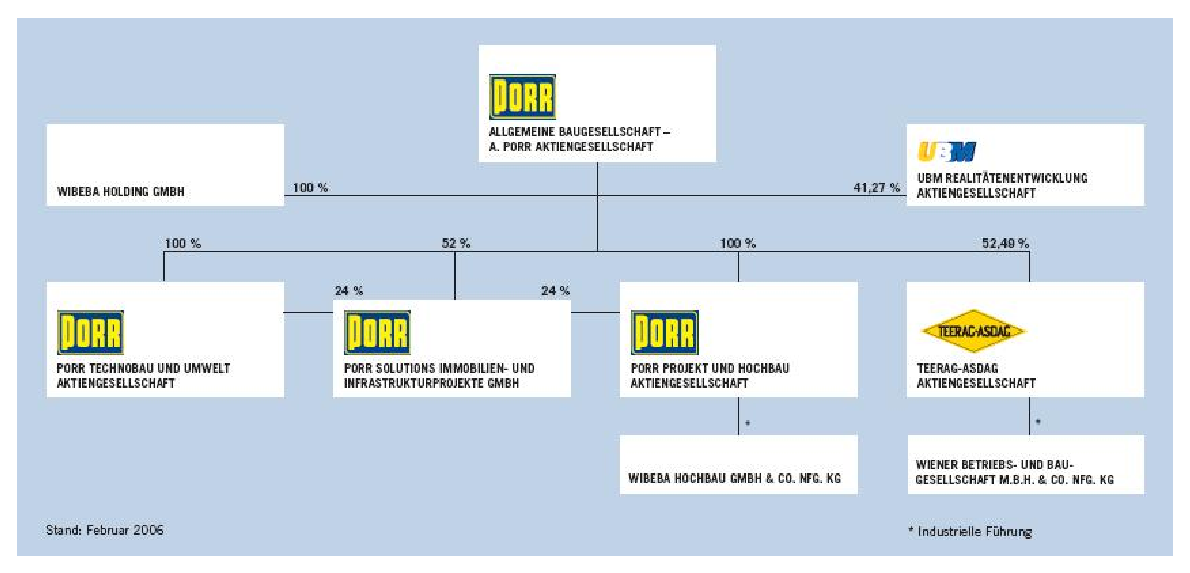
\includegraphics[width = \textwidth]{porr.eps}
	\caption{Porr Konzern�bersicht Quelle: \cite{porr}}
	\label{fig:porr}
\end{figure}


\subsection{Allgemeines zur Baubranche}
\label{sec:Allgemeines}

Die \emph{Bauindustrie} ist einer der wichtigsten Sektoren der �sterreichischen Wirtschaft. Einerseits waren im Jahre 2004   rund 21.600 Unternehmen �sterreichs im Bauwesen t�tig (Quelle:~\cite{branchenmonitor}) und andererseits liefert das Bauwesen einen Beitrag von rund sieben Prozent (15,7 Mrd. Euro) zum Bruttoinlandsprodukt.

Au�erdem spielen (�ffentliche) Bauinvestitionen eine gro�e Rolle. Diese stellen eine der effizientesten M�glichkeiten dar, um wachstums- und stabilit�tspolitische Zielsetzungen zu erreichen, indem die Konjunktur \"uber den Multiplikatoreffekt angekurbelt wird\footnote{Vgl. \cite{baujahr}}.

\subsubsection{Bauindustrie}
\label{sec:Bauindustrie}

\begin{figure}
\centering
\caption{Sparten der Bauindustrie, Quelle:~\cite{leitbetriebe}}
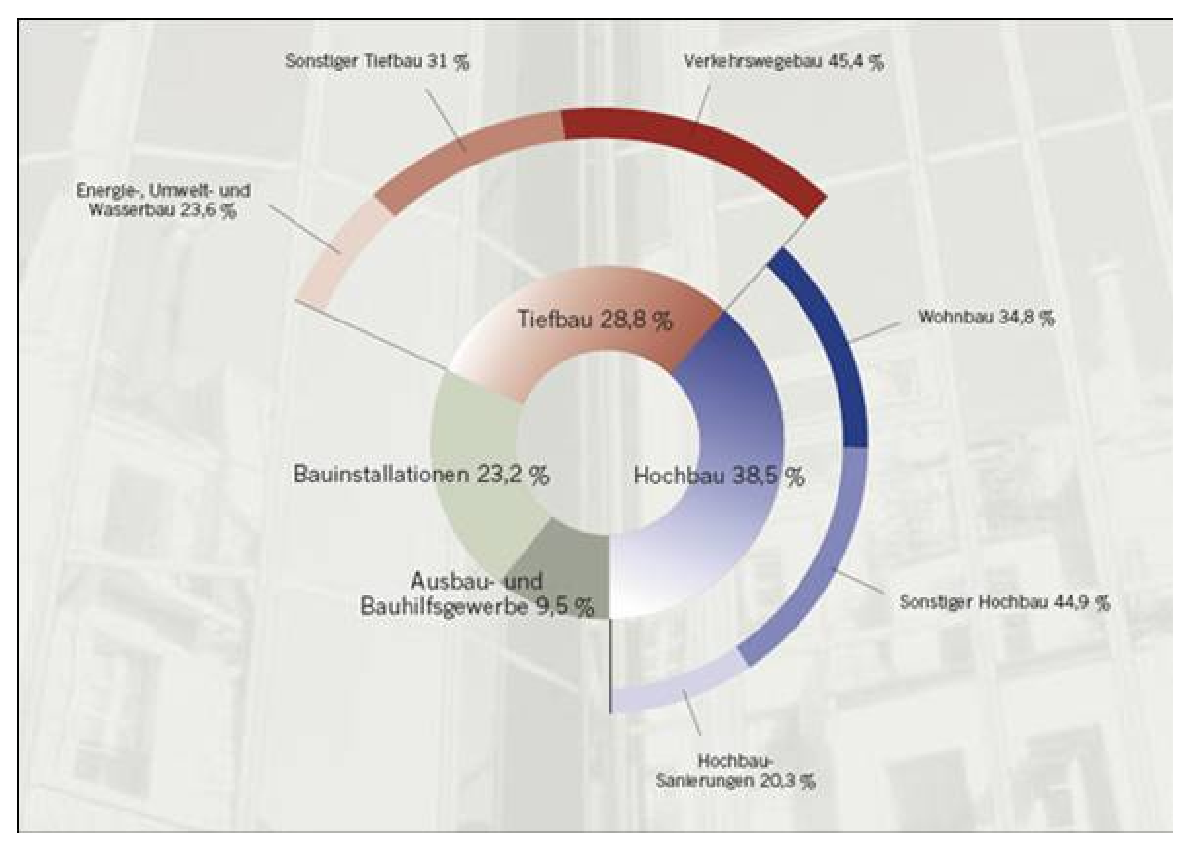
\includegraphics[width = 0.7\textwidth]{branche.eps}
\label{pic:Sparten}
%\cite{www.leitbetriebe.at}
\end{figure}

So beudeutend die Bauindustrie ist, so vielf�ltig sind auch ihre Sparten. Wie in Abbildung \ref{pic:Sparten} ersichtlich, gibt es die Sparten \emph{Hoch- und Tiefbau}, \emph{Ausbau- und Bauhilsgewerbe} sowie die Sparte \emph{Bauinstallationen}, wobei der Hochbau mit einem Produktionswert von \"uber 6 Mrd. Euro den gr��ten Bereich darstellt (Quelle:~\cite{baujahr}).

Nach den schwierigen Jahren 2001 und 2002 und der teilweisen positiven Entwicklung in 2003 und 2004 steigt der Optimismus seit 2005 wieder und es wird mit einem soliden Wachstum gerechnet. Auch die Konjunkturerholung Anfang 2006 wird neben der Sachg\"utererzeugung gr��tenteils der Bauwirtschaft zugeschrieben. Betriebe des Hoch- und Tiefbaus melden aufgrund eines erh�hten Bedarfs an Wohnungen eine g\"unstige Auftragslage, erwarten h�here Preise durchsetzen zu k�nnen und beabsichtigen Personal aufzunehmen. Ebenfalls g\"unstig ist die Auftragslage im Stra�en- und Schienenbau (Quelle:~\cite{AK}), wobei vor allem der Ausbau der Anbindungen an die neuen EU-Mitgliedstaaten ausschlaggebend ist.

\subsubsection{Konjunktur}
\label{sec:Konjunktur}

F\"ur das Jahr 2005 wurde von der \emph{Forschungsgesellschaft f\"ur Bauen, Wohnen und Planen} (FGW) f\"ur die gesamte Bauwirtschaft ein reales Wachstum des Produktionswertes um 1,3~\% prognostiziert. Die tragende St\"utze hierbei ist der Tiefbau mit Zuw�chsen von 4~\%, wohingegen es im Hochbau zur Stagnation kommt. Dies spiegelt sich auch im Baupreisindex nieder: Im Hochbau kam es einer Steigerung der Baukosten, wobei d�e Steigerung der Preise niedriger ausfiel. Dies ist ein Indiz f\"ur den starken Preiswettbewerb im Bauwesen.

Prognosen f\"ur 2006 �hneln den oben beschriebenen Werten. Jedoch konnte mit der Sicherung der Wohnbauf�rderung bis 2008 zumindest eine kleine F�rderung der Sparte Hochbau erzielt werden, daher rechnet das Wirtschaftsforschungsinstitut mit einem Wachstum von 1,4~\%. Tragend bleibt aber der Tiefbau mit einem Wachstum von 2,5~\%. Eine \"Ubersicht \"uber die Prognosen ist in Tabelle~\ref{table:wachstum} ersichtlich. 

Besonders zu betonen ist hierbei, dass vor allem im Bereich des Spezialtiefbaus mit 10 \% f\"ur 2005 ein hohes Wachstumspotential steckt. Im Jahre 2004 betrug das Wachstum in diesem Bereich sogar 25 \%.

\begin{table}
  \centering
  \caption{Bauproduktion nach Sparten, reale Ver�nderung gegen\"uber dem Vorjahr in Prozent (Prognosen 2005 - 2007), Quelle:~\cite{branchenmonitor}}
  \label{table:wachstum}
  \begin{tabular}{|l|r|r c r|}
    \hline
    & FGW && WIFO &\\
    & 2005 & 2005 & 2006 & 2007\\
    \hline
    Hochbau & 0,0 & 0,9 & 1,4 & 1,8\\
    ~~davon:&&&&\\
    ~~Wohnungsbau: & -1,7 & 0,6 & 0,9 & 1,6\\
    ~~Nutzbau: & 1,8 & 1,1 & 2,4 & 2,1\\
    ~~Modernisierung und Sanierung: & -0,8 & - &- &-\\
    Tiefbau &4,0 & 3,2 & 2,5 & 2,7\\
    ~~davon:&&&&\\
    ~~Rohrleitungs-und Kabeltiefbau & -4,1 & - & - &-\\
    ~~Stra�en- und Eisenbahnoberbau & 5,7 & - &- &-\\
    ~~Spezialbau &10,0 & -&-&-\\
    Hoch- und Tiebau gesamt & 1,6 & 1,5 & 1,7 & 2,0\\
    Bauhilfs- und Baunebengewerbe & 0,8 & - &- &-\\
    \hline
  \end{tabular}
\end{table}

%\newpage

\section{Branchenanalyse nach Porter}
\label{sec:Porter}

\subsection{Wettbewerb in der Branche}
\label{sec:Wettbewerb}

\subsubsection{Anzahl der Wettbewerber}
\label{sec:Anzahl}

Wie bereits erw�hnt gibt es mehr als 20.000~Unternehmen, die im Bauwesen t�tig sind. Hierbei war vor allem in den letzten Jahren ein \"uberm��iger Anstieg zu verzeichnen, n�mlich +~34~\% von 1997 bis 2004 (zum Vergleich: Industrie +~9~\%, Quelle:~\cite{AK}). Dies liegt allerdings daran, dass viele Ein-Personen-Gesellschaften gegr\"undet wurden, welche nicht als Konkurrenz f\"ur die \emph{A. PORR AG} angesehen werden k�nnen.

Auch kleinere Baugesellschaften mit Bauleistungen von unter 50~Mio.~Euro k�nnen aufgrund der Gr��enverh�ltnisse der \emph{A. PORR AG} nicht als direkte Wettbewerber angesehen werden. Vielmehr ist es so, dass sich die oftmals als Generalunternehmen agierende \emph{A. PORR AG} dieser kleinen Bauunternehmungen als Subunternehmen bedient.

Von der Wirtschaftskammer �sterreich (\cite{leitbetriebe})sowie im Bericht \cite{AK} wurde versucht, die beudeutensten Leitbetriebe der Bauwirtschaft �sterreichs zu identifizieren. Nach dieser Analyse sind die wichtigsten Konkurrenten f\"ur die \emph{A. PORR AG}, beurteilt nach ihrer erbrachten Bauleistung im Jahr 2005, die \emph{STRABAG AG, Wien}, die \emph{Alpine Mayreder BaugesmbH, Salzburg-Wals}, die \emph{SWIETELSKY Baugesellschaft m.b.H., Linz}, die \emph{Teerag-Asdag AG, Wien} (wobei die \emph{A. PORR AG} allerdings an der \emph{Teerag-Asdag AG, Wien} beteiligt ist) und die \emph{HABAU Hoch- und Tiefbau GmbH, Perg}. Eine detaillierte \"Ubersicht mit allen Unternehmen ist in Tabelle~\ref{table:uebersicht} im Appendix~\ref{sec:uebersicht} ersichtlich.

Die Konkurrenz dieser Unternehmen ist sehr gro�. Bei allen gr��eren Ausschreibungen bieten diese mit und sind somit unmittelbare Wettbewerber der \emph{A. PORR AG}. Vor allem bei Ausschreibungen des �ffentlichen Sektors ist dies deutlich bemerkbar, allerdings k�nnte der \"Ubergang vom Billigstbieter- zum Bestbieter-Prinzip (siehe Kapitel~\ref{sec:Barrieren}) wieder einen Vorteil f\"ur die \emph{A. PORR AG} darstellen.


\subsubsection{Differenzierung und Positionierung}
\label{sec:Differenzierung}

Zun�chst ist eine Differenzierung nach \emph{Kunden} n�tig. Die Kunden k�nnen in der Bauindustrie sehr unterschiedlich sein, n�mlich vom kleinen H�uslbauer bis hin zum Staat als Auftraggeber. Aufgrund des riesigen Verwaltungsapparates konzentriert sich die \emph{A. PORR AG} haupts�chlich auf gr��ere Projekte, die \emph{H�uslbauer} z�hlen somit nicht zu den Zielkunden. Dies k�nnte f\"ur die \emph{A. PORR AG} ein Problem darstellen, weil nur Gro�projekte angenommen werden k�nnen.

Der n�chste Schritt liegt in der Differenzierung nach Produkten. Hierbei ist gemeint, in welchen Sparten das Unternehmen t�tig ist (zB Hoch-, Tief- Stra�enbau usw.). Da die gro�en Unternehmen hier h�ufig als Generalunternehmen auftreten, m\"ussen sie alle Sparten abdecken. Dies f\"uhrt zwangsl�ufig dazu, dass nur einige wenige gro�e Unternehmen in der Branche sind, unter denen der Wettbewerb sehr hoch ist. Andererseits gibt es auch einige Unternehmen, die sich nur auf Spezialgebiete konzentrieren, wie beispielsweise die \emph{Gleitbau GmbH, Salzburg}, welche sich auf den Bau unter Verwendung von konischen und zylindrischen Gleitschalungstechniken konzentriert. Eine \"Ubersicht nach welchen Kriterien sich die �sterreichischen Leitbetriebe zu differenzieren versuchen, ist in Tabelle~\ref{table:Differenzierung} im Appendix~\ref{sec:diff} gegeben.

Weiters wird in der Branche h�ufig \emph{Qualit�t} als Positionierungsma�nahme genannt, wobei aber zu sagen ist, dass beinahe alle der in Tabelle~\ref{table:uebersicht} genannten Unternehmen Qualit�tsanforderungen nach den Normen \emph{ISO 9001}, \emph{ISO 9002}, \emph{ISO 14001} (Umweltmanagementsystem) und \emph{SCC**} (Arbeitssicherheits-Management-System) erf\"ullen bzw. sich bem\"uhen diese m�glichst bald zu erf\"uellen.  Qualit�t allein kann daher keine ausreichende Differenzierung im Markt darstellen.

Besondere Bedeutung kommt der Auswahl zu, in welchen M�rkten man sich positionieren will. Die \emph{A. PORR AG} konzentriert sich hierbei auf M�rkte der zehn neuen Mitgliedsstaaten der EU. Wie auch in Kapitel~\ref{sec:Marktwachstum} beschrieben, ist hier weiterhin ein hohes Wachstum in der Bauleistung zu erwarten. Die \emph{A. PORR AG} ist in diesen M�rkten bereits pr�sent und hat hier einen wesentlichen Vorteil gegen\"uber anderen Konkurrenten, die sich gr��tenteils auf die M�rkte in Zentraleuropa (bzw. sogar \"Ubersee) konzentrieren. Besonders profitieren k�nnte die \emph{A. PORR AG} hier vom Ausbau der Verkehrsanbindungen zwischen �sterreich und den Osteurop�ischen L�ndern.

Ein weiteres Differenzierungsmerkmal wird im Angebot von sogenannten \emph{Full Services} (von der Projektplanung bis zur tats�chlichen \"Ubergabe) gesehen. Jedoch muss gesagt werden, dass auch hier vor allem bei gro�en Projekten die Bauunternehmen h�ufig als Generalunternehmer auftreten. Dies \emph{muss} mehr oder weniger schon das Angebot von \emph{Full Services} inkludieren.

Die \emph{A. PORR AG} differenziert sich folgenderma�en von ihren Konkurrenten: Sie gibt an ein Spezialist in jeder Hinsicht zu sein und Spezialgebiete perfekt zu beherrschen, n�mlich von der Planung �ber die Fertigstellung bis hin zum Facility Management oder zur Verwertung. Auch langj�hrige  Erfahrung und Effizienz macht die \emph{A. PORR AG} besonders wettbewerbsf�hig.

%Weitere wichtige Positionierungsmerkmale der \emph{A. PORR AG} sind:
%
%\begin{itemize}
%\item Umfassendes Leistungsspektrum (Komplettanbieter in den Sparten Stra�en-, Kanal- und Umweltschutzbau)
%\item Reibungslose Koordination aller Unternehmensbereiche wodurch Projekte auch wesentlich schneller realisiert werden k�nnen
%\item Pr�senz in den Wachstumsm�rkten von Osteuropa
%\end{itemize}


\subsubsection{Marktwachstum}
\label{sec:Marktwachstum}

Die Situation in �sterreich wurde bereits im Kapitel~\ref{sec:Konjunktur} beschrieben. Es wird also mit einer Stagnation im Hochbau (trotz Sicherung der Wohnbauf�rderung bis 2008) und einem Wachstum im Tiefbau, vor allem im Spezialtiefbau gerechnet. In Deutschland gibt es wieder positive Signale einer ersten Erholung der Bauindustrie und im zentraleurop�ischen Raum wird in den n�chsten 10 bis 15 Jahren mit einem \"uberdurchschnittlichen Wachstum gerechnet.

Von besonderer Bedeutung ist aber, dass in den neuen EU-Mitgliedsstaaten mit einem Wachstum der Bauproduktion von \"uber 5~\% gerechnet wird. Da die \emph{A. PORR AG} in diesen M�rkten bereits pr�senter ist als andere gro�e (�sterreichische) Bauunternehmen, stellt dies einen immensen Wettbewerbsvorteil dar (Quelle:~\cite{porr}).

Weitere Prognosen besagen, dass der Kraftwerksbau in den n�chsten Jahren eine unvermeidliche Renaissance erleben wird. Weiters sollten private Investoren wieder vermehrt in B�ros und Industrieanlagen investieren. 

\subsubsection{Regulative Barrieren}
\label{sec:Barrieren}

In der Bauwirtschaft �ndern sich die Rahmenbedingungen st�ndig und das bedarf auch st�ndiger Regulierung durch staatliche Ma�nahmen. Im folgenden soll kurz auf einige aktuelle Ma�nahmen eingegangen werden:

Die EU strebt eine Harmonisierung der Regelungen des Bauwesens f\"ur alle Mitgliedsstaaten an, besonders bedrohend hierbei ist Umsetzung der \emph{Arbeitnehmerfreiz\"ugigkeit}. Bis 2006 wurde die Arbeitnehmerfreiz\"ugigkeit f\"ur die neuen EU-Mitgliedsstaaten sistiert. Jedoch kann die Zusischerung dieser Grundfreiheit zu einem Preisverfall im Lohnniveau f\"uhren. F\"ur die \emph{A. PORR AG} k�nnte dies aber einen Vorteil bedeuten, denn dadurch, dass sie bereits Filialen in den neuen Mitgliedsstaaten hat, k�nnte sie die billigeren Arbeitskr�fte auch f\"ur Projekte in �sterreich einsetzen.

Es stand kurz zur Diskussion, aufgrund der \"uberdurchschnittlichen Arbeitslosigkeit in der Bauindustrie (u. a. saisonell bedingt) den Beitrag zur Arbeitslosenversicherung f\"ur die Baubranche zu erh�hen. Die f\"uhrenden Unternehmen sehen diese Forderung allerdings als Polemie.

Die hohen Besch�ftigungszahlen in der Bauindustrie stellen allerdings ein gewaltiges politisches Machtpotential dar. W\"urde sich die \emph{A. PORR AG} beispielsweise aufgrund der Stagnation im Hochbau entschlie�en, diesen Bereich abzusto�en, h�tte dies viele Entlassungen zur Folge. Da dies aus volkswirtschaftlicher Sicht nicht erw\"unscht ist, wird der Staat ein jedes Unternehmen, das solche Vorhaben �u�ert, unter politischen Druck setzen.

Eine sehr gro�e Rolle spielt das \emph{Bundesvergabegesetz}. Bisher war es so, dass bei einer �ffentlichen Ausschreibung der Billigstbieter den Zuschlag bekommen hat. Hier soll nun ein neues Vergaberecht eingef\"uhrt werden, nach dem nicht der Billigst- sonder der \emph{Bestbieter} den Zuschlag erh�lt. % (\emph{\textbf{link zu stefan}}).

Auch hinsichtlich von Umweltvertr�glichkeitspr\"ufungen wird ein neues Verfahren angestrebt, welches bei der Pr\"ufung eine Erweiterung des Beteiligtenkreises vorsieht. Die bietet neue Verz�gerungspotentiale f\"ur die Fertigstellung von Bauvorhaben.

\subsubsection{Markenidentit�t}
\label{sec:Marken}

Markenidentit�t spielt keine allzu gro�e Bedeutung, denn schlie�lich erfolgt der Zuschlag bei gro�en Projekten immer nach dem Billigst- bzw. Bestbieterprinzip. Weiters hinzu kommt, dass alle gr��eren Bauunternehmen bereits ISO-Qualit�tszertifizierungen vorweisen k�nnen. Wichtig scheint aber zu sein, dass als Generalunternehmen mit Full-Service-Angeboten aufgetreten wird.

\subsection{Potentielle Mitbewerber}
\label{sec:Mitbewerber}

Der Markteintritt f�r potentielle Konkurrenten ist im Baugewerbe sehr schwierig. Alleine die extrem hohen Insolvenzzahlen in dieser Branche schrecken bereits einige ab. Andere Barrieren umfassen das n�tige Wissen/Know How, Kapital, Kunden und Mitarbeiter.

\subsubsection{Know How/Wissen}
\label{sec:Know How}

\"Reduzierung des einfachen Baugesch�fts, zugunsten einer Erh�hung des Anteils an komplexen Projekten, die weniger Konkurrenten ausf�hren k�nnen\" lautet eine der strategisches Sto�richtungen von \emph{A. PORR AG} (Quelle:~\cite{porr}). Wie an dieser Aussage schon zu erkennen ist, handelt es sich bei der \emph{A. PORR AG} um einen Full Service Anbieter mit einen sehr gro�en Know How. Genau dieses Wissen und die langj�hrige Erfahrung ist einer der Faktoren, welcher die \emph{A. PORR AG} vor neuen Konkurrenten sch�tzt. Die Kunden verlangen heute eine Betreuung von der Planung bis zum Betrieb und dies k�nnen nur wenige sehr gro�e Unternehmen anbieten, bzw. wird nur den erfahrenen Unternehmen zugetraut. Neue Marktteilnehmer sind nicht in der Lage Referenzen f�r teure, komplizierte Bauvorhaben vorzuweisen und daher ist es schwierig f�r diese Unternehmen Fu� zu fassen.

Durch die langj�hrige Erfahrung haben bestehende Unternehmen meist auch einen Kosten- und Qualit�tsvorsprung. Zu erkl�ren ist dies durch die steigende Routine, welche in der Projektplanung beginnt und in der Durchf�hrung endet. Somit k�nnen bestehende Unternehmen auf ihr Vorwissen bzw. vergangene Projektdaten zur�ckgreifen und haben einen enormen Informationsvorteil. Kosten und Dauer eines komplexen Bauvorhabens k�nnen von neuen Unternehmen nur schwer kalkuliert werden.

\subsubsection{Gr�ssenersparnis/Kapitalbedarf}
\label{sec:Kapital}

Mit einem Auftragsvolumen von �ber 2 Mrd. Euro besitzt die \emph{A. PORR AG} eine Gr��e, die sonst nur die \emph{STRABAG AG} erreicht. Somit kann davon ausgegangen werden, dass neue Konkurrenten nur durch langfristiges Wachstum oder Fusionen anderen Branchenteilnehmer entstehen k�nnten. Alleine diese Gr��e bringt Vorteile gegen�ber neuen Markteilnehmer. Zum Einen k�nnen sehr gro�e Projekte auch nur von den Branchenriesen durchgef�hrt werden, da nur diese das Kapital, Arbeitnehmer und Maschinen zur Verf�gung haben, um langj�hrige Projekte durchzustehen. Andererseits gibt es nat�rlich Kostenvorteile gegen�ber kleineren Unternehmen. Diese Skalenvorteile umfassen ein breites Spektrum
\begin{itemize}
\item Einkauf von Rohstoffen, G�tern und Maschinen
\item Effektivere Maschinennutzung durch geringere Leerzeiten
\item Spezialisierung der Mitarbeiter
\end{itemize}

Um Projekte wie Spezialtunnelbau, Autobahnbau und Hochh�user durchf�hren zu k�nnen, m�ssen neue Konkurrenten vor allem zu Beginn hohe Investitionskosten in Kauf nehmen. Daher vergr��ert sich das Risiko f�r neue Unternehmen enorm im Vergleich zu anderen Branchen. Auch dies stellt eine der Barrieren f�r m�gliche Konkurrenten dar.

\subsubsection{Ausschreibungen/Kunden}
\label{sec:Kunden}

Potentielle Konkurrenten m�ssen sich gegen die bestehenden, erfahrenen Unternehmen durchsetzen, um einen Auftrag bei den wenigen Kunden zu erhalten. Dies ist ein weiterer Faktor, der den Markteintritt erschwert, da diese Auftr�ge oft in sehr komplizierten, komplexen Ausschreibungsverfahren vergeben werden und hier neue Unternehmen durch die mangelnde Erfahrung Nachteile haben. Au�erdem kann es vorkommen, dass eine gewisse Loyalit�t vorhanden ist, so werden zufriedene Kunden bei teuren riskanten Projekten eher ungern den Gesch�ftspartner wechseln.

\subsubsection{Mitarbeiter/Fachkr�fte}
\label{sec:Mitarbeiter}

Ein weiteres Problem f�r neue Marktteilnehmer besteht darin, die n�tige Anzahl an f�higen Mitarbeitern zu finden. Dabei wird davon ausgegangen, dass vor allem gute Fachkr�fte meist bereits bei anderen Konkurrenten unter Vertrag stehen. 


\subsubsection{Regionale Vorteile}
\label{sec:Region}

Konkurrenten vom Ausland sind nur bedingt zu f�rchten, da das Risiko mit der Entfernung im Quadrat zunimmt (Quelle:~\cite{AK}). Jedoch profitieren die gro�en Gerneralunternehmen wie die \emph{A. PORR AG} von den billigen Subfirmen aus Osteuropa. Da die \emph{A. PORR AG} bereits in den Wachstumsm�rkten in Osteuropa pr�sent ist, wird es f\"ur neue Konkurrenten schwer, Marktanteile zu gewinnen.


\subsection{Substitute}
\label{sec:Substitute}

Das Baugewerbe ist eines der Gewerbe, welches nicht oder nur kaum ersetzt werden kann. Weiters handelt es sich um eine sehr gro�e Branche in der nur Teilbereiche durch neue Technologien substituiert werden. Daher hat PORR nur sehr wenig Konkurrenz von Anbietern von Ersatzg�tern.

\subsubsection{Ersatzg�ter im Hochbau}
\label{sec:SubHochbau}
Fertigteilbau und Systembau sind erw�hnenswerte Substitutionsg�ter im Bereich der privaten Bauwirtschaft. Es hier muss aber erw�hnt werden, dass PORR als Unternehmen vor allem im Hochhaus-, Infrastruktur- und Tunnelbau angesiedelt ist.

Verst�rkt wird in Zukunft auf die Umweltvertr�glichkeit der benutzen Werkstoffe geschaut. Daher werden leichter, entsorgbare Stoffe bevorzugt. Auch die Energieeffizienz des Geb�udes wird durch die steigenden Energiekosten immer wichtiger. PORR hat diesen Trend erkannt und betreibt eine eigene F\&E Abteilung. Die Gefahr besteht aber, dass in Zukunft hochtechnologische Teilbereiche des Bau (z.B.: Isolierung) nur mehr durch kleinere spezialisierte Subunternehmen durchgef�hrt werden. 

Holz und Stahlbaukonstruktionen m�ssen auch noch erw�hnt werden.


\subsubsection{Substitutionsgefahr im Tiefbau}
\label{sec:SubTiefbau}

Der Infrastrukturbau umfasst unter anderem Strassen-, Eisenbahn-, Flughafen-, Tunnel- und Br�ckenbau. All diese Bereiche werden durch die steigende Mobilit�t immer st�rker und �fter benutzt. Die Ersatzg�ter im Tiefbau sind zum Gro�teil andere G�ter im Tiefbau. So k�nnte z.B. ein Tunnel durch eine Strasse oder eine Br�cke durch einen Tunnel ersetzt werden.

Eine Substitutionsgefahr gibt es nur im weiteren Sinne. F�hren oder Schiffe k�nnten Br�cken ersetzen, jedoch geht der Trend eher in die umgekehrte Richtung. Die vielleicht gr��te Gefahr geht von extrem ansteigenden �lpreisen aus. Falls die Mobilit�t nicht mehr leistbar w�re, braucht man auch keine Infrastruktur ausbauen. 





\subsection{Ressourcen}
\label{sec:Ressourcen}


\subsubsection{Verhandlungsmacht Lieferanten}

Die Lieferanten spielen sowohl als Zulieferer als auch als Subunternehmer in der Baubranche eine wichtige Rolle. Wenn wir uns die Materialaufwandsquote\footnote{Vgl. \cite{oenb}} ansehen, so liegt diese bei gro�en Unternehmen, wie auch bei der \emph{A. PORR AG} im Median, n�mlich bei ca. 58,4~\% (2004). 

\paragraph{Produktdifferenzierung:}

Die Verhandlungsmacht der Lieferanten nimmt mit der Produktdifferenzierung zu. Da in der Baubranche aber oft eine sehr gro�e Anzahl von Rohstofflieferanten zur Verf�gung steht,  ist in diesem Bereich die Macht der Lieferanten nicht sehr gro�. Jedoch darf man nicht vergessen, dass es auch hier, gerade im Spezialtiefbau oder in Umwelttechnologiebau, Spezialzulieferer mit einem hohen Know How gibt. Diese Zulieferer haben nat�rlich gerade als Subunternehmer am Lieferantenmarkt eine gewisse Monopolstellung. Wie bei der \emph{A. PORR AG} und auch anderen Bauunternehmen werden diese Know-How-tr�chtigen Sparten oft selbst gehalten.

\paragraph{Umstellungskosten:}

Bei Gro�projekten arbeiten der Materiallieferant und auch der Subunternehmer sehr eng mit dem Generalunternehmer zusammen. Beispielsweise kann es vorkommen, dass beispielsweise der Lieferant von Beton direkt ein Mischwerk auf der Baustelle errichtet. Ein gut funktionierender Terminplan spielt eine zentralle Rolle bei Gro�projekten. Um den Zeitplan einzuhalten, werden bei Nichterf�llen auch Strafen (P�nalen) vereinbart. Dieses Risiko (Umstellungskosten) �bertr�gt der Generalunternehmer teilweise auf dem Subunternehmer.

\paragraph{Ersatzprodukte:}

Mit steigender Anzahl der Ersatzprodukte sinkt auch die Macht der Lieferanten. Wie schon in obigem Punkt erkl�rt, gibt es auch die M�glichkeit, gewisse Produkte je nach Gegebenheit selbst kurzfristig herzustellen. Dadurch ist nat�rlich auch in diesem Bereich der Lieferant unter Druck. Auch im Bereich von Subunternehmer gibt es, speziell im Hochbau, eine Vielzahl von Anbietern.

\paragraph{Auftragsvolumen:}

Das Auftragsvolumen spielt eine zentrale Rolle bei der Verhandlungsmacht der Unternehmen. Es ist klar, dass ein Konzern wie die \emph{A. PORR AG} eine starke Verhandlungsposition hat. Diese Verhandlungsposition gegen�ber kleinen Lieferanten oder Subunternehmern steigt mit der Gr��e von der \emph{A. PORR AG} in Zukunft weiter an.
 

\paragraph{Lieferantenkonzentration:}

Je gr��er die Lieferantenkonzentration ist, desto gr��er ist die Konkurrenz unter den Lieferanten und somit ger�t auch der Preis und die Verhandlungsmacht eines jeden Lieferanten unter Druck. In der Baubranche ist es oft so, dass in schlechteren Zeiten Kleinunternehmer als Subunternehmer bei Gro�projekten t�tig sind. Hierbei ist sich der Generalunternehmer seiner Verhandlungsmacht bewusst und die Subunternehmer sind oft dazu bereit, zu Herstellkosten anzubieten.


\paragraph{Vorw�rtsintegration:}

Bei Gro�projekten besteht keine Gefahr, dass die Lieferanten(Subunternehmer) als Konkurrenten auftreten. Dies deshalb nicht, weil sie  Gro�projekte von der Logistik und Finanzierungsseite nicht alleine bew�ltigen k�nnten. Daher teilt sich der Markt bei Gro�projekten im �ffentlichen oder auch privaten Sektor eine geringe Zahl von Unternehmen.
Weiters ist es einem Matrialzulieferer auch nicht m�glich, direkt sein Produkt an den Kunden zu verkaufen. Da ja der Kunde nicht daran interessiert ist, die Baulogistik und das oft damit verbundene Risiko selbst zu tragen. Deshalb werden Gro�projekte meist Arbeitsgemeinschaften (ARGE) oder gro�en einzelnen Unternehmen �bergeben.




\subsubsection{Verhandlungsmacht Arbeitskr�fte}

Arbeitskr�fte sind in einem Gewerbebetrieb (Produktionsbetrieb) eines der wichtigsten Assets, das den Firmenerfolg pr�gt. Der durchschnittliche prozentuelle Anteil an Arbeitskr�ften am Gesamtumsatz liegt in der Baubranche bei ca. 28~\%.\footnote{Vgl. \cite{oenb}}

Die \emph{A. PORR AG} hat ca. 10.000 Mitarbeiter. Diese Anzahl ist von 2003 auf 2004 ca. um 9~\% gestiegen\footnote{Vgl. \cite{porr} Seite 58 ff}. Dies kommt aufgrund der guten Auftragslage in Zentral- und Osteuropa. 

Die Verhandlungsmacht in der Baubranche ist bei den Arbeitern teilweise sehr gering. Im Bereich von Hilfskr�ften ist ein �berangebot vorhanden (Ost�ffnung). Diese billigen Arbeitskr�fte hatten jedoch auf dem �sterreichischen Arbeitsmarkt noch keine Arbeitserlaubnis\footnote{Vgl. \cite{arbeiter}}, zumindest bis zum 30. April 2006. Da aber die \emph{A. PORR AG} schon lange am osteurop�ischen Markt Fu� gefasst hat, stellt diese Tatsache kein Problem dar. 
Qualit�t zu g�nstigem Preis ist ein Erfolgsfaktor, ebenso wie gut ausgebildete Fachkr�fte. In diesem Bereich wird es immer schwieriger, gutes Personal zu finden.

\subsubsection{Verhandlungsmacht Kapital}

Da die Baubranche eine kapitalintensive Branche (Vorfinanzierung) darstellt, spielt die Finanzierungsseite eine zentrale Rolle, die zum Erfolg oder Misserfolg beitr�gt.

Wenn man die Marktmacht der Kapitalgeber beschreiben will, so kann man sagen, dass diese bei kleinen Unternehmen sehr hoch ist und mit der Gr��e des Unternehmens abnimmt. Dies deshalb, weil mit steigender Gr��e die wirtschaftliche Wichtigkeit und auch das Finanzierungsvolumen zunimmt. Durch die hohe Fremdfinanzierung sind oft Banken somit stark mit den Unternehmen verstrickt oder sogar vielleicht an diesen beteiligt. Es entsteht somit oft eine gegenseitige Abh�ngigkeitsstruktur. 


\subsection{Kunden}
\label{sec:Kunden}

\subsubsection{Kundenkonzentration - Kundenvolumen}
Derzeit befindet sich die Baubranche auf einem H�henflug (hohes
Kundenvolumen im Hochbau). Es gibt
Wohnbauf�rderungen (in Wien bis 2008 gesichert), die eine starke
Kundenkonzentration, vorallem in Ballungsr�umen, hervorruft. Ob sich
dieser Trend mittelfristig
fortsetzen wird kann noch nicht gesagt werden. Es wird auch des
�fteren vom Platzen der Immobilienblase gesprochen, die sich vor allem
im B�rohaussegment aufstaut, gesprochen. Trotz ausgezeichneter
Auftragslage 2006 kann man nicht davon ausgehen, dass es in 3-5 Jahren
auch der Fall sein wird. Daher wird bis dahin die Verhandlungsmacht
eher zu den Kunden wandern, da das Kundenvolumen sp�rbar abnehmen wird
(Ende des Ostbooms?).
Im Spezialtiefbau zeigt sich ein anderes Bild. Hier ist das
Kundenvolumen sehr gering, das wird auch in Zukunft so
bleiben. Jedoch, wie vorher schon gezeigt, ist der Wettbewerb um diese
Kunden auch geringer, denn es gibt nicht viele Unternehmen, die in
diesem Bereich t�tig sind. Der Trend in diesem Segment ist steigend
(vor allem wenn man die Auslandsnachfrage mitber�cksichtigt). Im Inland
sind hier einige Projekte im Laufen bzw. in Planung (Koralmtunnel,
Semmeringtunnel, ...).

\subsubsection{Ersatzprodukte}
Im Hochbausegment ist der Trend zu Fertigteilh�usern erkennbar. Man
sollte vielleicht erw�gen auf diesen Zug aufzuspringen. Trotzdem
bleibt in der Baubranche eine Tendenz zu anderen Technologien
aus (siehe oben). Hier sollte sich auch in den n�chsten Jahren nichts Gravierendes
�ndern. Vorallem der Hochbausektor sollte wie schon erw�hnt
abgesch�pft und als Cashcow verwendet werden.

\subsubsection{F�higkeit zur R�ckwertsintegration}
Dies ist beinahe nicht gegeben. Es besteht maximal die Gefahr das
kleinere Kundensegmente (Bereich Eigenheime) ihre Projekte selbst
durchf�hren. Man kann jedoch davon ausgehen, dass dies keinen Einfluss
auf die Verhandlungsmacht haben wird, weil dies hier ein sehr kleiner
Bereich ist und bleiben wird. Im Tiefbau und vorallem im
Spezialtiefbau ist R�ckwertsintegration beinahe ausgeschlossen. Dieses
Segment ist daher als �u�erst positiv f�r \emph{A. PORR AG} zu beurteilen.

\subsubsection{Preis}
Im privaten Sektor ist ein starker Preiskampf zu sehen. Die Kunden
haben hier eine gr��ere Verhandlungsmacht, trotz gro�er Nachfrage. Es
gibt viele kleine, regionale Anbieter. Diese haben somit einen kleinen
Kostenvorteil. Die Gewinnmargen sind hier beschr�nkt. Man muss sich
hier mit hervorstechender Qualit�t einen guten Namen machen.
Bei den �ffentlichen Auftr�gen bzw. Gro�auftr�gen ist aufgrund der
wenigen gro�en Player die Verhandlungsmacht der Kunden
eingeschr�nkt. Volkswirtschaftlich kann man auch von einer gewissen
Oligopolstellung sprechen. Die gro�en Player bestimmen die Preise und
teilen sich die Auftr�ge auf. Die \emph{A. PORR AG} spielt in dieser Liga mit und das
sollte sich in den n�chsten Jahren auch nicht �ndern.

\subsubsection{Gefahrenpotentiale}
Im Hochbausektor wird sich in den n�chsten Jahren einiges
�ndern. Steigende Zinsen und daher ein R�ckgang der Investitionen wird
sich in diesem Segment stark auswirken. Kleine Baufirmen werden davon
st�rker betroffen sein als gr��ere (aufgrund der Gr��envorteile). Es
wird eine Zeit der \textit{Ernte} eintreten. Investmentfonds stehen
nach einem H�henflug vor einer schwierigen Phase. Auf jeden Fall wird sich
das Verh�ltnis Abnehmer zu Anbieter �ndern. Weniger Abnehmer werden
vielen Anbietern Gegen�berstehen.
D.h., es wird bessere Qualit�t zu niedrigerem Preis verlangt werden. Die
Verhandlungsmacht wird dem Kunden zugesprochen werden m�ssen. Eine gute
Marke wird hier von Vorteil sein. Bei der \emph{A. PORR AG} ist das so und wird sich in
absehbarer Zeit nicht �ndern.
Im Tiefbau ist dieser Trend aufgrund der stark �ffentlich gepr�gten
Auftr�ge nicht zu sehen.

\subsubsection{�ffentliche Auftr�ge}

Wie wir schon mehrmals  er�rtert
haben, besteht ein reger Wettbewerb der einzelnen Unternehmen um
Kundschaft. Sei es durch die gr��eren Konzerne wie \emph{A. PORR AG} und \emph{STRABAG AG},
sei es durch kleineren, aber regional pr�senteren
Unternehmen.Im Hochbau dominieren viele
regionale Anbieter den Markt. Die gr��eren Konzerne sind hier auf
gr��ere Auftr�ge angewiesen, wo man als sogenannte Generalunternehmen
fungiert. Eine enge Kooperation mit diesen
Anbietern ist hier w�nschenswert, um �ber die Dynamik in diesem
Segment nicht den Anschluss zu verlieren.

Entspannter ist die Lage im speziellen Tiefbau.
Hier kann man direkt mit dem Kunden in Kontakt treten und
zwar auf h�chster Ebene. Denn meist handelt es sich bei den
Auftraggebern um einen Staat oder ein Bundesland. Bei �ffentlichen
Ausschreibungen gibt es ein geregeltes Vergaberecht und somit ist die
Verhandlungsst�rke der Abnehmer nebens�chlich, da nach objektiven
Kriterien entschieden wird (Bestpreis- oder Bestbieterzuschlag).
Hier geht der Trend zur Vergabe nach dem Bestbieterprinzip. Die
Konzerne sind hier klar im Vorteil.

Generell ist das Abnehmerfeld beim Tiefbau allgemein recht
�berschaubar (bezogen auf einen Staat). Aufgrund der langj�hrigen Erfahrung
mit der Abwicklung von �ffentlichen Auftr�gen kann die \emph{A. PORR AG} in diesem
Bereich gr��tm�gliche Effektivit�t aufweisen. Ein weiteres Plus in
diesem Bereich ist, dass sich die  \emph{A. PORR AG} durch viele, mit h�chster
Zufriedenheit durchgef�hrte Auftr�ge, als qualit�tsorientiertes
Unternehmen etabliert hat.

%\newpage

\section{Bewertung und Zukunftsbild}
\label{sec:Bewertung}

\begin{table}[tbp]
  \centering
  \caption{Bewertung}
  \label{table:Bewertung}
  \begin{tabular}{|l|c|c|}
    \hline
    \begin{table}[tbp]
  \centering
  \caption{Bewertung}
  \label{table:Bewertung}
  \begin{tabular}{|l|c|c|}
    \hline
    \begin{table}[tbp]
  \centering
  \caption{Bewertung}
  \label{table:Bewertung}
  \begin{tabular}{|l|c|c|}
    \hline
    \input{bewertung.txt}
    \hline  
  \end{tabular}
\end{table}

Tabelle~\ref{table:Bewertung} gibt eine \"Ubersicht \"uber die Bewertung der einzelnen Punkte der Branchenanalyse. Hierbei wurde nach dem Schulnotensystem bewertet.

Der Wettbewerb in der Branche ist zwar stark, jedoch kann sich die \emph{A. PORR AG} in diesem Konkurrenzkampf gut behaupten. In Zukunft wird die \emph{A. PORR AG} durch ihre Konzentration auf die osteurop�ischen M�rkte im Wettbewerbkampf profitieren.

Hinsichtlich dem Markteintritt neuer Wettbewerber besteht aufgrund des hohen Kapitalbedarfes und des n�tigen Know-Hows keine gr��ere Gefahr. In Zukunft k�nnte sich der derzeitige Marktvorteil (durch den fr\"uhen Markteintritt) in Osteuropa schw�cher auswirken, deshalb die schlechtere Prognose.

Bei der Substitutionsgefahr durch Ersatzprodukte ist in der Baubranche
eine differenzierte Betrachtung n�tig: Im Hochbau ist die Gefahr durch
Stahl-, Holz-, Ferteil-, Systembau usw. gegeben, im Tiefbau hingegen
gibt es kaum Alternativen.

Aufgrund der Gr��e der \emph{A. PORR AG} besitzt sie gegen\"uber ihren
Lieferanten eine sehr gro�e Verhandlungsmacht. Diese wird durch die
Ost-Expansion weiter ausgebaut.

Aufgrund des abzusehenden R\"uckgangs beim Kundenvolumen gibt es eine
Tendenz zu wachsender Verhandlungsmacht bei den Kunden. Dies betrifft
haupts�chlich den privaten Sektor, welcher gr��tenteils den Hochbau
betrifft. Weiters sind steigende Zinsen zu ber\"ucksichtigen, welche
sicherlich Auswirkungen auf Investitionen in der Bauindustrie haben
werden.

In Summe ist die Wettbewerbssituation f\"ur die \emph{A. PORR AG} zufriedenstellend. Unsere Prognose weist eine sehr leicht fallende Tendenz auf, allerdings muss hier gesagt werden, dass keine Gewichtung der einzelnen Teilbereiche vorgenommen wurde, beispielsweise fiel der Punkt Harmonisierung gleich schwer ins Gewicht wie das Marktwachstum in Osteuropa.
    \hline  
  \end{tabular}
\end{table}

Tabelle~\ref{table:Bewertung} gibt eine \"Ubersicht \"uber die Bewertung der einzelnen Punkte der Branchenanalyse. Hierbei wurde nach dem Schulnotensystem bewertet.

Der Wettbewerb in der Branche ist zwar stark, jedoch kann sich die \emph{A. PORR AG} in diesem Konkurrenzkampf gut behaupten. In Zukunft wird die \emph{A. PORR AG} durch ihre Konzentration auf die osteurop�ischen M�rkte im Wettbewerbkampf profitieren.

Hinsichtlich dem Markteintritt neuer Wettbewerber besteht aufgrund des hohen Kapitalbedarfes und des n�tigen Know-Hows keine gr��ere Gefahr. In Zukunft k�nnte sich der derzeitige Marktvorteil (durch den fr\"uhen Markteintritt) in Osteuropa schw�cher auswirken, deshalb die schlechtere Prognose.

Bei der Substitutionsgefahr durch Ersatzprodukte ist in der Baubranche
eine differenzierte Betrachtung n�tig: Im Hochbau ist die Gefahr durch
Stahl-, Holz-, Ferteil-, Systembau usw. gegeben, im Tiefbau hingegen
gibt es kaum Alternativen.

Aufgrund der Gr��e der \emph{A. PORR AG} besitzt sie gegen\"uber ihren
Lieferanten eine sehr gro�e Verhandlungsmacht. Diese wird durch die
Ost-Expansion weiter ausgebaut.

Aufgrund des abzusehenden R\"uckgangs beim Kundenvolumen gibt es eine
Tendenz zu wachsender Verhandlungsmacht bei den Kunden. Dies betrifft
haupts�chlich den privaten Sektor, welcher gr��tenteils den Hochbau
betrifft. Weiters sind steigende Zinsen zu ber\"ucksichtigen, welche
sicherlich Auswirkungen auf Investitionen in der Bauindustrie haben
werden.

In Summe ist die Wettbewerbssituation f\"ur die \emph{A. PORR AG} zufriedenstellend. Unsere Prognose weist eine sehr leicht fallende Tendenz auf, allerdings muss hier gesagt werden, dass keine Gewichtung der einzelnen Teilbereiche vorgenommen wurde, beispielsweise fiel der Punkt Harmonisierung gleich schwer ins Gewicht wie das Marktwachstum in Osteuropa.
    \hline  
  \end{tabular}
\end{table}

Tabelle~\ref{table:Bewertung} gibt eine \"Ubersicht \"uber die Bewertung der einzelnen Punkte der Branchenanalyse. Hierbei wurde nach dem Schulnotensystem bewertet.

Der Wettbewerb in der Branche ist zwar stark, jedoch kann sich die \emph{A. PORR AG} in diesem Konkurrenzkampf gut behaupten. In Zukunft wird die \emph{A. PORR AG} durch ihre Konzentration auf die osteurop�ischen M�rkte im Wettbewerbkampf profitieren.

Hinsichtlich dem Markteintritt neuer Wettbewerber besteht aufgrund des hohen Kapitalbedarfes und des n�tigen Know-Hows keine gr��ere Gefahr. In Zukunft k�nnte sich der derzeitige Marktvorteil (durch den fr\"uhen Markteintritt) in Osteuropa schw�cher auswirken, deshalb die schlechtere Prognose.

Bei der Substitutionsgefahr durch Ersatzprodukte ist in der Baubranche
eine differenzierte Betrachtung n�tig: Im Hochbau ist die Gefahr durch
Stahl-, Holz-, Ferteil-, Systembau usw. gegeben, im Tiefbau hingegen
gibt es kaum Alternativen.

Aufgrund der Gr��e der \emph{A. PORR AG} besitzt sie gegen\"uber ihren
Lieferanten eine sehr gro�e Verhandlungsmacht. Diese wird durch die
Ost-Expansion weiter ausgebaut.

Aufgrund des abzusehenden R\"uckgangs beim Kundenvolumen gibt es eine
Tendenz zu wachsender Verhandlungsmacht bei den Kunden. Dies betrifft
haupts�chlich den privaten Sektor, welcher gr��tenteils den Hochbau
betrifft. Weiters sind steigende Zinsen zu ber\"ucksichtigen, welche
sicherlich Auswirkungen auf Investitionen in der Bauindustrie haben
werden.

In Summe ist die Wettbewerbssituation f\"ur die \emph{A. PORR AG} zufriedenstellend. Unsere Prognose weist eine sehr leicht fallende Tendenz auf, allerdings muss hier gesagt werden, dass keine Gewichtung der einzelnen Teilbereiche vorgenommen wurde, beispielsweise fiel der Punkt Harmonisierung gleich schwer ins Gewicht wie das Marktwachstum in Osteuropa.


\newpage
\section{Zusammenfassung}
\label{sec:Zusammenfassung}

Aus der obigen Analyse geht hervor, dass sich die \emph{A. PORR AG} vor allem auf die Bereiche Tiefbau und Spezialtiefbau konzentrieren soll. Ausschlaggebend hierf\"ur ist der zuk\"unftige Bedarf an Infrastruktur in Osteuropa. Au�erdem sollte der gro�e Know-How-Vorsprung im Bereich Spezialtiefbau ausgebaut werden.

Die Sparte Hochbau liefert zwar derzeit noch gute Ertr�ge, aber in Zukunft wird ein h�rterer Wettbewerb erwartet. Au�erdem besteht gerade im Hochbau die Gefahr durch Substitutionsg\"uter.


\bibliographystyle{plainnat}
\bibliography{bibfile}

%\newpage
\appendix

\section{Appendix}
\label{sec:Appendix}

\begin{table}[t]
  %\centering
  \caption{\"Ubersicht \"uber Leitbetriebe der Bauindustrie}
  \label{table:uebersicht}
  \begin{tabular}{|l|r|r|r |l|}
    \hline

    \begin{table}[t]
  %\centering
  \caption{\"Ubersicht \"uber Leitbetriebe der Bauindustrie}
  \label{table:uebersicht}
  \begin{tabular}{|l|r|r|r |l|}
    \hline

    \begin{table}[t]
  %\centering
  \caption{\"Ubersicht \"uber Leitbetriebe der Bauindustrie}
  \label{table:uebersicht}
  \begin{tabular}{|l|r|r|r |l|}
    \hline

    \input{uebersicht.txt}

    \hline


  \end{tabular}
\end{table}

    \hline


  \end{tabular}
\end{table}

    \hline


  \end{tabular}
\end{table}
\label{table:uebersicht}

\begin{table}
  \centering
  \caption{Differenzierung der Leitbetriebe}
  \label{table:Differenzierung}
  \begin{tabular}{|l|l|}
    \hline
			
\begin{table}
  \centering
  \caption{Differenzierung der Leitbetriebe}
  \label{table:Differenzierung}
  \begin{tabular}{|l|l|}
    \hline
			
\begin{table}
  \centering
  \caption{Differenzierung der Leitbetriebe}
  \label{table:Differenzierung}
  \begin{tabular}{|l|l|}
    \hline
			
\input{differenzierung1.txt}

  \end{tabular}
\end{table}


  \end{tabular}
\end{table}


  \end{tabular}
\end{table}

\label{table:Differenzierung1}

\begin{table}
  \centering
  \caption{Fortsetzung zu Tabelle~\ref{table:Differenzierung}: Differenzierung der Leitbetriebe}
  \label{table:FortsetzungDifferenzierung}
  \begin{tabular}{|l|l|}
    \hline
			
\begin{table}
  \centering
  \caption{Fortsetzung zu Tabelle~\ref{table:Differenzierung}: Differenzierung der Leitbetriebe}
  \label{table:FortsetzungDifferenzierung}
  \begin{tabular}{|l|l|}
    \hline
			
\begin{table}
  \centering
  \caption{Fortsetzung zu Tabelle~\ref{table:Differenzierung}: Differenzierung der Leitbetriebe}
  \label{table:FortsetzungDifferenzierung}
  \begin{tabular}{|l|l|}
    \hline
			
\input{differenzierung2.txt}
\hline
  \end{tabular}
\end{table}

\hline
  \end{tabular}
\end{table}

\hline
  \end{tabular}
\end{table}

\label{table:Differenzierung2}

\end{document}
